%% bare_conf.tex
%% V1.4b
%% 2015/08/26
%% by Michael Shell
%% See:
%% http://www.michaelshell.org/
%% for current contact information.
%%
%% This is a skeleton file demonstrating the use of IEEEtran.cls
%% (requires IEEEtran.cls version 1.8b or later) with an IEEE
%% conference paper.
%%
%% Support sites:
%% http://www.michaelshell.org/tex/ieeetran/
%% http://www.ctan.org/pkg/ieeetran
%% and
%% http://www.ieee.org/

%%*************************************************************************
%% Legal Notice:
%% This code is offered as-is without any warranty either expressed or
%% implied; without even the implied warranty of MERCHANTABILITY or
%% FITNESS FOR A PARTICULAR PURPOSE!
%% User assumes all risk.
%% In no event shall the IEEE or any contributor to this code be liable for
%% any damages or losses, including, but not limited to, incidental,
%% consequential, or any other damages, resulting from the use or misuse
%% of any information contained here.
%%
%% All comments are the opinions of their respective authors and are not
%% necessarily endorsed by the IEEE.https://www.overleaf.com/project/5e568e914222610001394a75
%%
%% This work is distributed under the LaTeX Project Public License (LPPL)
%% ( http://www.latex-project.org/ ) version 1.3, and may be freely used,
%% distributed and modified. A copy of the LPPL, version 1.3, is included
%% in the base LaTeX documentation of all distributions of LaTeX released
%% 2003/12/01 or later.
%% Retain all contribution notices and credits.
%% ** Modified files should be clearly indicated as such, including  **
%% ** renaming them and changing author support contact information. **
%%*************************************************************************


% *** Authors should verify (and, if needed, correct) their LaTeX system  ***
% *** with the testflow diagnostic prior to trusting their LaTeX platform ***
% *** with production work. The IEEE's font choices and paper sizes can   ***
% *** trigger bugs that do not appear when using other class files.       ***                          ***
% The testflow support page is at:
% http://www.michaelshell.org/tex/testflow/



\documentclass[a4paper,conference]{IEEEtran}
\usepackage{graphicx}
\usepackage{amsmath}
\graphicspath{ {./images/} }

% Some Computer Society conferences also require the compsoc mode option,
% but others use the standard conference format.
%
% If IEEEtran.cls has not been installed into the LaTeX system files,
% manually specify the path to it like:
% \documentclass[conference]{../sty/IEEEtran}





% Some very useful LaTeX packages include:
% (uncomment the ones you want to load)


% *** MISC UTILITY PACKAGES ***
%
%\usepackage{ifpdf}
% Heiko Oberdiek's ifpdf.sty is very useful if you need conditional
% compilation based on whether the output is pdf or dvi.
% usage:
% \ifpdf
%   % pdf code
% \else
%   % dvi code
% \fi
% The latest version of ifpdf.sty can be obtained from:
% http://www.ctan.org/pkg/ifpdf
% Also, note that IEEEtran.cls V1.7 and later provides a builtin
% \ifCLASSINFOpdf conditional that works the same way.
% When switching from latex to pdflatex and vice-versa, the compiler may
% have to be run twice to clear warning/error messages.






% *** CITATION PACKAGES ***
%
%\usepackage{cite}
% cite.sty was written by Donald Arseneau
% V1.6 and later of IEEEtran pre-defines the format of the cite.sty package
% \cite{} output to follow that of the IEEE. Loading the cite package will
% result in citation numbers being automatically sorted and properly
% "compressed/ranged". e.g., [1], [9], [2], [7], [5], [6] without using
% cite.sty will become [1], [2], [5]--[7], [9] using cite.sty. cite.sty's
% \cite will automatically add leading space, if needed. Use cite.sty's
% noadjust option (cite.sty V3.8 and later) if you want to turn this off
% such as if a citation ever needs to be enclosed in parenthesis.
% cite.sty is already installed on most LaTeX systems. Be sure and use
% version 5.0 (2009-03-20) and later if using hyperref.sty.
% The latest version can be obtained at:
% http://www.ctan.org/pkg/cite
% The documentation is contained in the cite.sty file itself.






% *** GRAPHICS RELATED PACKAGES ***
%
\ifCLASSINFOpdf
  % \usepackage[pdftex]{graphicx}
  % declare the path(s) where your graphic files are
  % \graphicspath{{../pdf/}{../jpeg/}}
  % and their extensions so you won't have to specify these with
  % every instance of \includegraphics
  % \DeclareGraphicsExtensions{.pdf,.jpeg,.png}
\else
  % or other class option (dvipsone, dvipdf, if not using dvips). graphicx
  % will default to the driver specified in the system graphics.cfg if no
  % driver is specified.
  % \usepackage[dvips]{graphicx}
  % declare the path(s) where your graphic files are
  % \graphicspath{{../eps/}}
  % and their extensions so you won't have to specify these with
  % every instance of \includegraphics
  % \DeclareGraphicsExtensions{.eps}
\fi
% graphicx was written by David Carlisle and Sebastian Rahtz. It is
% required if you want graphics, photos, etc. graphicx.sty is already
% installed on most LaTeX systems. The latest version and documentation
% can be obtained at:
% http://www.ctan.org/pkg/graphicx
% Another good source of documentation is "Using Imported Graphics in
% LaTeX2e" by Keith Reckdahl which can be found at:
% http://www.ctan.org/pkg/epslatex
%
% latex, and pdflatex in dvi mode, support graphics in encapsulated
% postscript (.eps) format. pdflatex in pdf mode supports graphics
% in .pdf, .jpeg, .png and .mps (metapost) formats. Users should ensure
% that all non-photo figures use a vector format (.eps, .pdf, .mps) and
% not a bitmapped formats (.jpeg, .png). The IEEE frowns on bitmapped formats
% which can result in "jaggedy"/blurry rendering of lines and letters as
% well as large increases in file sizes.
%
% You can find documentation about the pdfTeX application at:
% http://www.tug.org/applications/pdftex





% *** MATH PACKAGES ***
%
\usepackage{bm}
% A popular package from the American Mathematical Society that provides
% many useful and powerful commands for dealing with mathematics.
%
% Note that the amsmath package sets \interdisplaylinepenalty to 10000
% thus preventing page breaks from occurring within multiline equations. Use:
%\interdisplaylinepenalty=2500
% after loading amsmath to restore such page breaks as IEEEtran.cls normally
% does. amsmath.sty is already installed on most LaTeX systems. The latest
% version and documentation can be obtained at:
% http://www.ctan.org/pkg/amsmath





% *** SPECIALIZED LIST PACKAGES ***
%
%\usepackage{algorithmic}
% algorithmic.sty was written by Peter Williams and Rogerio Brito.
% This package provides an algorithmic environment fo describing algorithms.
% You can use the algorithmic environment in-text or within a figure
% environment to provide for a floating algorithm. Do NOT use the algorithm
% floating environment provided by algorithm.sty (by the same authors) or
% algorithm2e.sty (by Christophe Fiorio) as the IEEE does not use dedicated
% algorithm float types and packages that provide these will not provide
% correct IEEE style captions. The latest version and documentation of
% algorithmic.sty can be obtained at:
% http://www.ctan.org/pkg/algorithms
% Also of interest may be the (relatively newer and more customizable)
% algorithmicx.sty package by Szasz Janos:
% http://www.ctan.org/pkg/algorithmicx




% *** ALIGNMENT PACKAGES ***
%
%\usepackage{array}
% Frank Mittelbach's and David Carlisle's array.sty patches and improves
% the standard LaTeX2e array and tabular environments to provide better
% appearance and additional user controls. As the default LaTeX2e table
% generation code is lacking to the point of almost being broken with
% respect to the quality of the end results, all users are strongly
% advised to use an enhanced (at the very least that provided by array.sty)
% set of table tools. array.sty is already installed on most systems. The
% latest version and documentation can be obtained at:
% http://www.ctan.org/pkg/array


% IEEEtran contains the IEEEeqnarray family of commands that can be used to
% generate multiline equations as well as matrices, tables, etc., of high
% quality.




% *** SUBFIGURE PACKAGES ***
%\ifCLASSOPTIONcompsoc
%  \usepackage[caption=false,font=normalsize,labelfont=sf,textfont=sf]{subfig}
%\else
%  \usepackage[caption=false,font=footnotesize]{subfig}
%\fi
% subfig.sty, written by Steven Douglas Cochran, is the modern replacement
% for subfigure.sty, the latter of which is no longer maintained and is
% incompatible with some LaTeX packages including fixltx2e. However,
% subfig.sty requires and automatically loads Axel Sommerfeldt's caption.sty
% which will override IEEEtran.cls' handling of captions and this will result
% in non-IEEE style figure/table captions. To prevent this problem, be sure
% and invoke subfig.sty's "caption=false" package option (available since
% subfig.sty version 1.3, 2005/06/28) as this is will preserve IEEEtran.cls
% handling of captions.
% Note that the Computer Society format requires a larger sans serif font
% than the serif footnote size font used in traditional IEEE formatting
% and thus the need to invoke different subfig.sty package options depending
% on whether compsoc mode has been enabled.
%
% The latest version and documentation of subfig.sty can be obtained at:
% http://www.ctan.org/pkg/subfig




% *** FLOAT PACKAGES ***
%
%\usepackage{fixltx2e}
% fixltx2e, the successor to the earlier fix2col.sty, was written by
% Frank Mittelbach and David Carlisle. This package corrects a few problems
% in the LaTeX2e kernel, the most notable of which is that in current
% LaTeX2e releases, the ordering of single and double column floats is not
% guaranteed to be preserved. Thus, an unpatched LaTeX2e can allow a
% single column figure to be placed prior to an earlier double column
% figure.
% Be aware that LaTeX2e kernels dated 2015 and later have fixltx2e.sty's
% corrections already built into the system in which case a warning will
% be issued if an attempt is made to load fixltx2e.sty as it is no longer
% needed.
% The latest version and documentation can be found at:
% http://www.ctan.org/pkg/fixltx2e


%\usepackage{stfloats}
% stfloats.sty was written by Sigitas Tolusis. This package gives LaTeX2e
% the ability to do double column floats at the bottom of the page as well
% as the top. (e.g., "\begin{figure*}[!b]" is not normally possible in
% LaTeX2e). It also provides a command:
%\fnbelowfloat
% to enable the placement of footnotes below bottom floats (the standard
% LaTeX2e kernel puts them above bottom floats). This is an invasive package
% which rewrites many portions of the LaTeX2e float routines. It may not work
% with other packages that modify the LaTeX2e float routines. The latest
% version and documentation can be obtained at:
% http://www.ctan.org/pkg/stfloats
% Do not use the stfloats baselinefloat ability as the IEEE does not allow
% \baselineskip to stretch. Authors submitting work to the IEEE should note
% that the IEEE rarely uses double column equations and that authors should try
% to avoid such use. Do not be tempted to use the cuted.sty or midfloat.sty
% packages (also by Sigitas Tolusis) as the IEEE does not format its papers in
% such ways.
% Do not attempt to use stfloats with fixltx2e as they are incompatible.
% Instead, use Morten Hogholm'a dblfloatfix which combines the features
% of both fixltx2e and stfloats:
%
% \usepackage{dblfloatfix}
% The latest version can be found at:
% http://www.ctan.org/pkg/dblfloatfix




% *** PDF, URL AND HYPERLINK PACKAGES ***
%
%\usepackage{url}
% url.sty was written by Donald Arseneau. It provides better support for
% handling and breaking URLs. url.sty is already installed on most LaTeX
% systems. The latest version and documentation can be obtained at:
% http://www.ctan.org/pkg/url
% Basically, \url{my_url_here}.




% *** Do not adjust lengths that control margins, column widths, etc. ***
% *** Do not use packages that alter fonts (such as pslatex).         ***
% There should be no need to do such things with IEEEtran.cls V1.6 and later.
% (Unless specifically asked to do so by the journal or conference you plan
% to submit to, of course. )


% correct bad hyphenation here
\hyphenation{op-tical net-works semi-conduc-tor}


\begin{document}
%
% paper title
% Titles are generally capitalized except for words such as a, an, and, as,
% at, but, by, for, in, nor, of, on, or, the, to and up, which are usually
% not capitalized unless they are the first or last word of the title.
% Linebreaks \\ can be used within to get better formatting as desired.
% Do not put math or special symbols in the title.
\title{Deep transformation models: Tackling complex regression problems with neural network based transformation models}



% author names and affiliations
% use a multiple column layout for up to three different
% affiliations
\author{\IEEEauthorblockN{Beate Sick*}
\IEEEauthorblockA{UZH and ZHAW\\
Email: sick@zhaw.ch}
\and
\IEEEauthorblockN{Torsten Hothorn}
\IEEEauthorblockA{UZH\\
Email: torsten.hothorn@uzh.ch}
\and
\IEEEauthorblockN{Oliver Dürr*}
\IEEEauthorblockA{HTWG\\
Email: oliver.duerr@htwg-konstanz.de}
}

% conference papers do not typically use \thanks and this command
% is locked out in conference mode. If really needed, such as for
% the acknowledgment of grants, issue a \IEEEoverridecommandlockouts
% after \documentclass

% for over three affiliations, or if they all won't fit within the width
% of the page, use this alternative format:
%
%\author{\IEEEauthorblockN{Michael Shell\IEEEauthorrefmark{1},
%Homer Simpson\IEEEauthorrefmark{2},
%James Kirk\IEEEauthorrefmark{3},
%Montgomery Scott\IEEEauthorrefmark{3} and
%Eldon Tyrell\IEEEauthorrefmark{4}}
%\IEEEauthorblockA{\IEEEauthorrefmark{1}School of Electrical and Computer Engineering\\
%Georgia Institute of Technology,
%Atlanta, Georgia 30332--0250\\ Email: see http://www.michaelshell.org/contact.html}
%\IEEEauthorblockA{\IEEEauthorrefmark{2}Twentieth Century Fox, Springfield, USA\\
%Email: homer@thesimpsons.com}
%\IEEEauthorblockA{\IEEEauthorrefmark{3}Starfleet Academy, San Francisco, California 96678-2391\\
%Telephone: (800) 555--1212, Fax: (888) 555--1212}
%\IEEEauthorblockA{\IEEEauthorrefmark{4}Tyrell Inc., 123 Replicant Street, Los Angeles, California 90210--4321}}




% use for special paper notices
%\IEEEspecialpapernotice{(Invited Paper)}




% make the title area
\maketitle

% As a general rule, do not put math, special symbols or citations
% in the abstract
\begin{abstract}
Deep neural networks are known for their outstanding accurate predictions in supervised learning for complex and high dimensional data such as images. Still, in many real world applications uncertainty remains due to variability inherent in the data and the non-deterministic character of the tasks. Especially if crucial decisions are based on the predictions, it is essential to capture their uncertainties. However, regression in deep learning is predominantly used to just predict the mean. Here, we present a deep learning transformation model which estimates a complete conditional probability distribution, the best way to capture uncertainty in probabilistic models.

Our method combines ideas from a statistical transformation model (most likely transformation) with recent transformation models from deep learning (normalizing flows) to predict complex outcome distributions. The core of the method is a parametrized transformation function which can be trained with the usual maximum likelihood framework. This method can be combined with existing deep learning architectures. 

For small machine learning benchmark datasets, we report state of the art performance for most dataset and partly even outperform it. We further show that our method works for complex input data like images employing a CNN architecture.
 

\end{abstract}

% no keywords
% For peer review papers, you can put extra information on the cover
% page as needed:
% \ifCLASSOPTIONpeerreview
% \begin{center} \bfseries EDICS Category: 3-BBND \end{center}
% \fi
%
% For peerreview papers, this IEEEtran command inserts a page break and
% creates the second title. It will be ignored for other modes.
\IEEEpeerreviewmaketitle

\section{Introduction}
Deep learning (DL) models are known for their outstanding performance in prediction tasks when working with complex data. Especially in high dimensional perceptual tasks like image or sound classification DL outperforms traditional models \cite{Lecun2015}. For deep  classification tasks the networks are almost always treated as probabilistic models, where the output nodes (after softmax) are interpreted as the probability for the different classes. This conditional probability distribution (CPD) is also known as multinomial distribution. The networks are trained by minimizing the negative log-likelihood (NLL) of the observed classes under the predicted CPD. DL is also successfully used in regression tasks with complex data. In regression tasks DL models, however, are often not used in a probabilistic setting and yield only a point estimate for the expected value of the outcome. 

Many real world applications are not deterministic, in a sense that a whole range of outcome values are possible, potentially with different probabilities. In this setting, we need a model that does not only predict a point estimate but the whole outcome distribution conditioned on the input.  

In many applications a Gaussian CPD is assumed, often with the additional assumption that the variance of the Gaussian does not depend on the input $x$ (homoscedastic). In the Gaussian homoscedastic cases only one node in the last layer is needed and interpreted as the conditional $\hat{\mu}_{x}$ of the CPD $N(\hat{\mu}_{x}, \sigma^2)$. In this case the NLL is proportional to the mean squared error $\frac{1}{n} \sum_{i=1}^n(y_i - \hat{\mu}_{x_i})^2$, which is one of the best known loss functions in regression. Minimizing the loss function yields the maximum likelihood estimate of the parameter $\mu$ of the Gaussian CPD. The parameter $\sigma^2$ of the CPD is estimated from the resulting residuals $r_i=y_i - \hat{\mu}_{x_i}$, an approach that only works in the homoscedastic case. In case of non-constant variance, a second output node is needed which controls the variance.  

The likelihood approach generalizes to other types of CPDs, especially if the CPD is known to be a member of a parameterized distribution family, such as the Poissonian with rate parameter $\lambda_x}$ which is conditioned on the input $x$. 

\section{Related Work}
A simple parameterized distribution like the Gaussian or an other member of the exponential family is sometimes not flexible enough to model the conditional distribution of the outcome in real-world applications.  A straightforward approach to model more flexible CPDs is to use a mixtures of simple distributions. Mixtures of Gaussian, where the mixing coefficients and the parameters of the individual Gaussians are controlled by a neural network, are known as neural density mixture networks and have been used for a long time \cite{Bishop1994}.

Another way to achieve more complex distributions is to average over many different CPDs, where each  CPD is a simple distribution. This approach is taken by  ensemble models \cite{NIPS2017_7219} or alternatively Bayesian models. A Bayesian deep learning treatment for regression has been done by MC-Dropout \cite{Gal2015}, \cite{Gal2017b} 

Transformation models take a different approach to model a flexible distributions. Here, a parameterized bijective transformation function is learned that transforms between a the flexibel distribution and a simple base distribution such as a Gaussian. The likelihood of the data can be easily determined from the base distribution after transformation using the change of variable formula. This allows to determined the parameters of the transformation using the maximum likelihood principle. A historic side remark: the same principle was used in old days when statisticians worked with tables of the standard normal distribution to get likelihoods for a non-standard normal distribution. 



\subsection{Normalizing flows}
On the “deep learning” side the normalizing flows (NF) have recently successfully been used to model complex probability distributions of high-dimensional data \cite{Rezende2015}. See  \cite{Papamakarios2019} for an extensive review. A typical NF transforms from a simple base distribution with density $f_z(z)$ (often a Gaussian) to a more complex target distribution $f_y(y)$ for the outcome variable $y$. This is done with parameterized transformation function $h_{\theta}^{-1}(z)$.

A NF usually consists of a chain of simple transformations interleaved with non-linear activation functions. To achieve a bijective overall transformation, it is sufficient that each transformation in the chain is be bijective. The bijectivity is usually enforced by choosing a strictly monotone increasing transformation. A simple but efficient and often used transformation consists of a scale $a(z)$ and shift terms $b(z)$:

\begin{equation}
    y=h_\theta^{-1}(z) = a(z) \cdot z - b(z)
\end{equation}

To enforce the required monotony of $a(z) $needs to be positive. Note that the density in y after transformation is determined by the change of variable formula: 

\begin{equation}
f_y(y)=f_z(h_\theta(y))|h_\theta'(y)|
\end{equation}

The Jacobi-Determinant $|h_\theta'(y)|$ ensures that $f_y(y)$ is again normalized. The parameters in the transformation function, here  $(a(z), b(z))$ are controlled by the output of a neural network carefully designed so that the Jacobi-Determinant is easy to calculate \cite{Papamakarios2019}. To ensure that $a(z)$ is positive, the output of a network $\tilde a(z)$ is transformed e.g. by $a(z)=\exp(\tilde a(z))$. By chaining several such transformations with non-linear activation functions in between, a target distributions can be achieved which has not only another mean and spread, but also another shape than the base distribution.

NFs are very successfully used in modeling high dimensional unconditional distributions.  They can be used for data generation, like creating photorealistic samples human faces \cite{Kingma2018}. However, little research is done yet with respect to using NF in a regression-like setting, where the distribution of a low-dimensional variable $y$ is modeled conditioned on a possible high-dimensional variable $x$. Only very recently, NF have been used in such a setting. In the approach of \cite{Rothfuss} a neural network controls the parameters of a chain of normalizing flow, consisting of scale and shift terms combined with additional simple radial flows. 


\subsection{Most Likely Transformation}
On the other side, transformation models have a long tradition in classical statistics, dating back to the 1960’s starting with the seminal work of Box and Cox on transformation models \cite{Box1964}. Recently this approach has been generalized to a very flexible class of  transformations called most likely transformation (MLT) \cite{Hothorn2018}. The MLT models a complex distribution $p_y(y|x)$ of a one-dimensional random variable $y$ conditioned on a possible high-dimensional variable $x$. While multivariate extensions of the framework exists \cite{Klein2019}, we restrict our treatment to the practically important case of a univariate response $y$. As in normalizing flows the fitting is done by learning a parameterized bijective transformation $h_\vartheta(y|x)$ of $(y|x)$ to a simple distribution $(z|x)=h_\vartheta(y|x) \sim \Phi$, such as a standard Gaussian $\Phi=N(0,1)$. The parameters are determined using the maximum likelihood principle to the training data. The change of variable theorem allows computing the probability density $f_y(y|x)$ of the complicated distribution from the simple distribution $f_z(z|x)$ via:

\begin{equation}
    f_y(y|x)=f_z(h(y|x)) \cdot |h'(y|x)|    
\end{equation}

As in the NF, the factor $|h'(y)|$ ensures the normalization of $f_y(y|x)$. The key insight of the MLT method is to use a flexible class of polynomials, e.g. the Bernstein polynomials, to approximate the transformation function.
\begin{equation}
    h_\vartheta^{\tt MLT}(\tilde y) = \sum_{i=0}^M {\tt Be_i}(\tilde{y}) \frac{\vartheta_i(x_i)}{M+1}
\end{equation}
where $\tilde  y\in [0,1]$. The core of this transformation is the Bernstein Basis of order $M$, generated by the $M+1$ Beta-densities  ${\tt Be_i}(\tilde{y}) = f_{i+1, M-i+1}(\tilde y)$. It is known that the Bernstein polynomials are very flexible basis functions and uniformly approximate every function in $y \in [0,1]$, see \cite{Hothorn2018} for a further discussion. The second reason for the choice of the Bernstein basis is that in order for $h_\vartheta(\tilde y)$ to be bijective, a strict monotone transformation of $\tilde y$ is required. A strict increase of a polynomial of Bernstein Basis can be guaranteed by simply enforcing that the coefficients of the polynomial are increasing, i.e. $\vartheta_0 < \vartheta_1 < \ldots < \vartheta_M$.

TODO (Torsten): add some words about Shift Model as special case which is less flexible but provide some interpretability


\section{Method}
In the following, we combine the ideas of NF parameterized by neural networks and MLT. 
Our model consists of a chain of four transformations constructing the parametric transformation function:

\begin{equation}
\label{eq:MLT}
    z = h_\theta(y) = f_{3, \alpha, \beta } \circ f_{2, \vartheta_0, \ldots, \vartheta_M} \circ \sigma \circ f_{1, a, b}(y)
\end{equation}

Only the sigmoid transformation $\sigma$ has no parameters, whereas $ f_1, f_2, f_3$ have learnable parameters. In a regression task we allow in our flexible model all parameters to change with $x$. We use neural networks to control the parameters (see Figure \ref{fig:NN}). We describe the chain of flows going from the untransformed variable $y$ to the standard normally distributed variable $z$. The MLT approach based on Bernstein polynomials needs a target variable which is limited between $[0,1]$. For our model, we do not want to apriori define a fixed upper and lower bound of $y$ to restrict its range. Instead, we transform in a first flow $f_1$, $y$ to the required range of $[0,1]$. This is done by a scaled and shift transformation followed by a sigmoid function via:

\begin{equation}
    f_1: \;\; \tilde{y} = \sigma(a(x) \cdot y - b(x))
\end{equation}

The scale and shift parameters $(a, b)$ are allowed to depend on $x$ and are controlled by the output of two neural networks with input $x$. In order to enforce $f_1$ to be monotonicaly increasing, we need to restrict  $a(x) > 0$. This is enforced by a softplus activation of the last neuron (see figure \ref{fig:NN}). 

The second transformation $f_2$ is the MLT transformation from Equation \ref{eq:MLT} consisting of a Bernstein polynomial with $M+1$ parameters  $\vartheta_0 , \vartheta_1,\ldots \vartheta_M$  which can depend on $x$ and are controlled by a NN with input $x$ and as many output nodes as we have parameter. To ensure a monotone increasing $f_2$, we enforce the above discussed condition $\vartheta_0 < \vartheta_1 < \ldots < \vartheta_M$ by choosing $\vartheta_k=\vartheta_{k-1} + \exp(\vartheta_k)$ for $k>0$ and $l_k$ being the k-th output of the network. We set $\vartheta_0=l_0$ (see Figure \ref{fig:NN}).

The final flow in the chain $f_3$ is again a scale and shift transformation into the range of the standard normal. The parameters $(\alpha, \beta)$ are also allowed to depend on x and are controlled again by NNs, where the softplus transformation is used to guarantee a positive $x$ (see Figure \ref{fig:NN}). First experiments showed that the third flow is not necessary for the performance but accelerate the training. 

The total transformation $ h_\theta(y): y \rightarrow z $ is given by chaining the the three transformations resulting in (see figure trafo):

\begin{equation}
\begin{split}
    z_x &= h_{\theta(x)}(y) = \alpha(x) \cdot h_{\vartheta(x)}^{\tt MLT}(\tilde y) - \beta(x) \\\
    &= \alpha(x) \left( \sum_{i=0}^M {\tt Be_i}(\sigma(a(x) \cdot y - b(x)) \frac{\vartheta_i(x_i)}{M+1} \right) - \beta(x)
\end{split}
\end{equation}

\begin{figure}
\centering
\includegraphics[width=.8\linewidth]{architecture.pdf}
\caption{The network architecture of our model which is trained end to end starting with the input x yielding the conditional parameters of the transformation function. The dashed CNN part is only used in case of image input data. If some parameters should be not allowed to depend on x, the respective NN gets a constant number (one) as input. }
\label{fig:NN}
\end{figure}

Our model has been implemented in R using Keras, TensorFlow, and TensorFlow Probability and can be found at: XXXXX.


\begin{figure}
\centering
\includegraphics[width=.8\linewidth]{images/method.pdf}
\caption{Upper: TODO: make a nice figure illustrating the chain of flow and the resulting transformation function along with the base and target densitiy}
\label{fig:fig_trafo}
\end{figure}

\section{Experiments}
In order to demonstrate the capacity of our proposed approach, we performed three different experiments.

\subsection{1 Dimensional Toy Data}
We use simulated toy data sets with a single feature and a single target variable to illustrate some properties of the proposed transformation model. In the first example the data generating process is given by imposing Exponential noise with increasing amplitude one a linear increasing sinusoidal (see Figure \ref{fig:fig_sin}). For some x-values two fitted CPDs are shown, one resulting from our NN based transformation model with $M=10$ (solid line) and one from a less flexible linear-shift transformation model (dotted) Figure \ref{fig:fig_sin} clearly demonstrates that the complex transformation model  can, in contrast to the simple linear-shift transformation, cope with an non-monotone x-dependency of the variance. To quantify the goodness of fit, we us the negative log-likelihood (NLL) of the data (smaller is better), which is -2.00 for the complex and -0.85 for the simple transformation model. 


\begin{figure}
\centering
\includegraphics[width=.99\linewidth]{images/1D_Toy_sin.pdf}
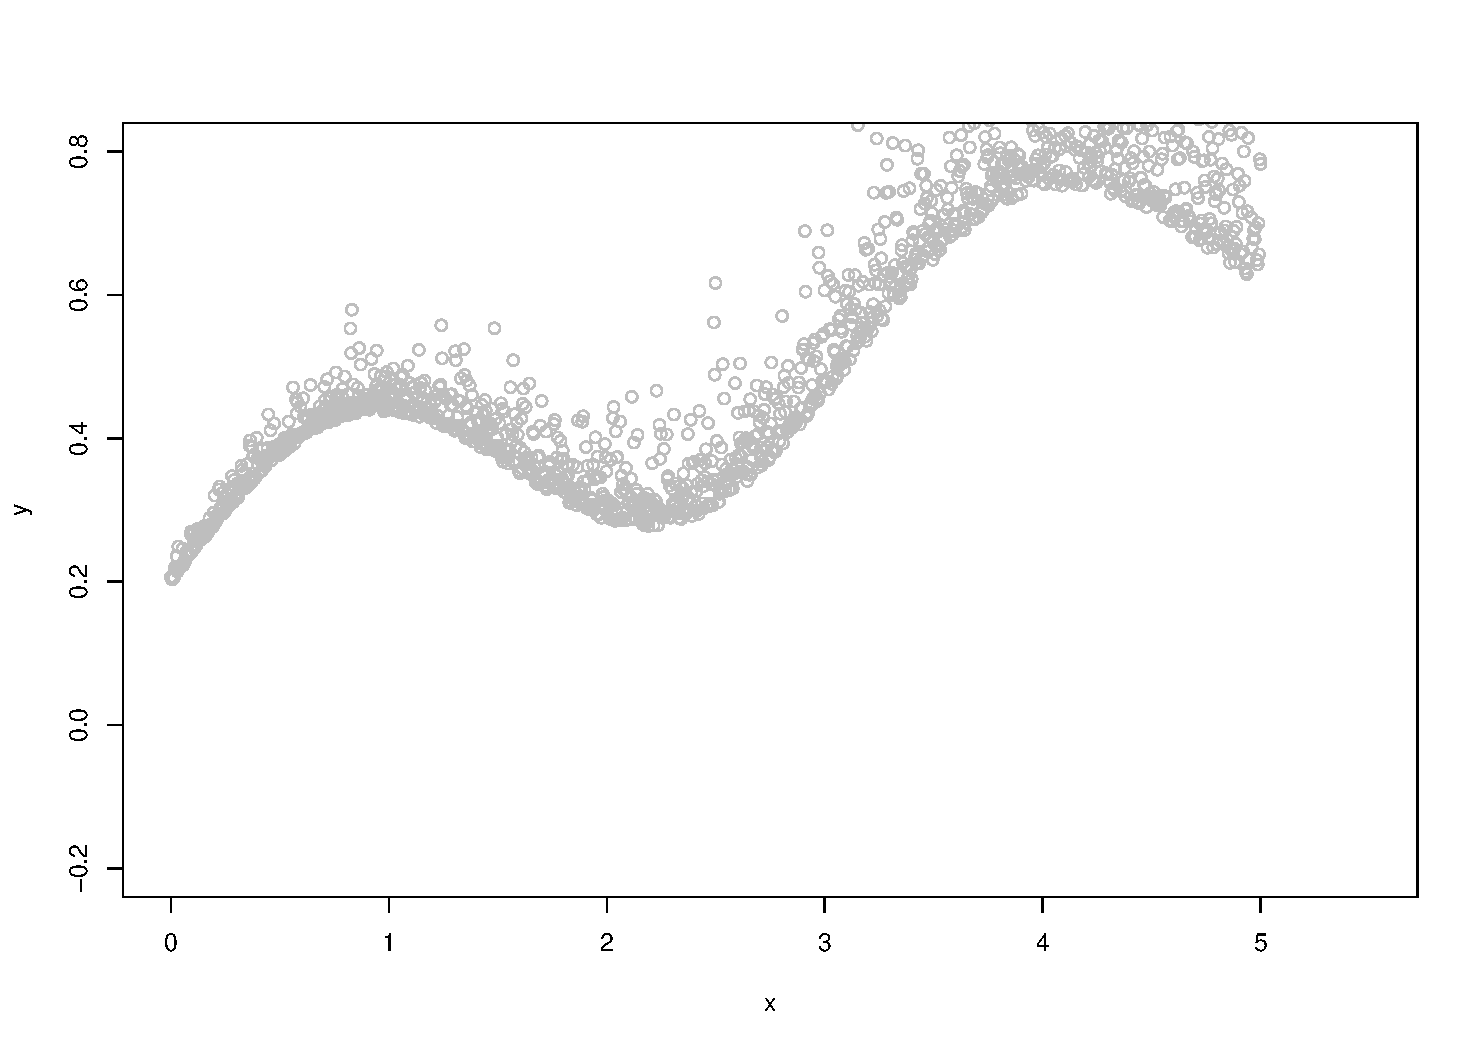
\includegraphics[width=.99\linewidth]{images/1D_toy_2l.pdf}
\caption{Simple one-dimensional toy example with complex outcome distributions. Training data is shown as grey points and the estimated CPDs for the linear shift model and the proposed DL\_MLT method are shown for two data generating process as a dashed and solid lines, respectively. In the upper panel in addition the true CPD of the data generating process is shown (dotted line). The CPDs have been scaled down for plotting.
}
\label{fig:fig_sin}
\end{figure}

The second example, shown on the lower panel of figure \ref{fig:fig_sin}, is a challenging bimodal distribution in which the spread between the modes strongly depends on $x$ but the conditional mean of the outcome $y$ does not depend on $x$. Both models can capture the bimodal shape of the CPD, but the linear shift model is not flexible enough to adapt its bimodal CPD with changing $x$. The proposed flexible transformation model is able to also take the $x$ dependency of the spread between the modes of the distribution into account. 




\subsection{UCI-Benchmark data sets}
\begin{table*}[!t]
% increase table row spacing, adjust to taste
\renewcommand{\arraystretch}{1.3}
% if using array.sty, it might be a good idea to tweak the value of
% \extrarowheight as needed to properly center the text within the cells
\caption{Comparison of prediction performance (test NLL, smaller is better)  on regression benchmark UCI datasets. The best method for each dataset is bolded, as are those with standard errors that overlap with the standard errors of the best method.}
\label{table_example}


\centering
%% Some packages, such as MDW tools, offer better commands for making tables
%% than the plain LaTeX2e tabular which is used here.
\begin{tabular}{rcccccccc}
Data Set & N & DL\_MLT & NGBoost & MC Dropout & Deep Ensembles & Gaussian Process & MDN & NFN \\
Boston & 506 & 2.42 $\pm$ 0.050 & 2.43 $\pm$ 0.15 & 2.46 $\pm$0.25 & 2.41 $\pm$0.25 & 2.37 $\pm$0.24 & 2.49 $\pm$ 0.11 & 2.48 $\pm$0.11 \\
Concrete & 1030 & 3.29 $\pm$ 0.02 & 3.04 $\pm$ 0.17 & 3.04 $\pm$0.09 & 3.06 $\pm$0.18 & 3.03 $\pm$0.11 & 3.09 $\pm$ 0.08 & 3.03 $\pm$0.13 \\
Energy & 768 & 1.06 $\pm$ 0.09 & 0.60 $\pm$ 0.45 & 1.99 $\pm$0.09 & 1.38 $\pm$0.22 & 0.66 $\pm$0.17 & 1.04 $\pm$ 0.09 & 1.21 $\pm$0.08 \\
Kin8nm & 8192 & -0.99 $\pm$ 0.01 & -0.49 $\pm$ 0.02 & -0.95 $\pm$0.03 & -1.20 $\pm$0.02 & -1.11 $\pm$0.03 & NA & NA \\
Naval & 11934 & -6.54 $\pm$ 0.03 & -5.34$\pm$ 0.04 & -3.80 $\pm$0.05 & -5.63 $\pm$0.05 & -4.98 $\pm$0.02 & NA & NA \\
Power & 9568 & 2.85 $\pm$ 0.005 & 2.79 $\pm$ 0.11 & 2.80 $\pm$0.05 & 2.79 $\pm$0.04 & 2.81 $\pm$0.05 & NA & NA \\
Protein & 45730 & 2.63 $\pm$ 0.006 & 2.81 $\pm$ 0.03 & 2.89 $\pm$0.01 & 2.83 $\pm$0.02 & 2.89 $\pm$0.02 & NA & NA \\
Wine & 1588 & 0.67 $\pm$ 0.028 & 0.91 $\pm$ 0.06 & 0.93 $\pm$0.06 & 0.94 $\pm$0.12 & 0.95 $\pm$0.06 & NA & NA \\
Yacht & 308 & 0.004 $\pm$ 0.046 & 0.20 $\pm$ 0.26 & 1.55 $\pm$0.12 & 1.18 $\pm$0.21 & 0.10 $\pm$0.26 & NA & NA \\
\end{tabular}


\end{table*}

To compare the predictive performance of our NN based transformation model with other state-of-the-art methods, we use nine well established benchmark data sets (see table bench) from the UCI Machine Learning Repository. Shown is our approach (Deep\_MLT), NGBoost \cite{Duan2020}, MC Dropout \cite{Gal2015}, Deep Ensembles \cite{NIPS2017_7219}, Gaussian Process \cite{Duan}, noise regularized Gaussian Mixture Density Networks (MDN) and normalizing flows networks (NFN) \cite{Rothfuss}. As hyperparameters, we used $M=10$ for all datasets and a L2-regularisation constants of 0.01 for the smaller datasets  (Yacht, Energy, Concrete, and Boston) no regularisation was used in the other datasets.
To quantify the prediction performance, we use the negative log-likelihood (NLL) on test data. The NLL is a strictly proper score that takes its minimum only if and only if the predicted CPD matches the true CPD \cite{TODO} and is therefore often used when comparing the performance of probabilistic models.


In order to compare with other state-of-art models, we follow the protocol from Hernandez and Lobato \cite{Hernandez-Lobato2015} that was also employed by Gal \cite{Gal2015}. For validating our method, the benchmark data sets were split in several folds containing training data (90 percent) and test-data (10 percent).  We downloaded the specific folds as used in  \cite{Gal2015} from https://github.com/yaringal/DropoutUncertaintyExps. We determined the hyperparameters of our model using 80 percent of the training data, keeping 20 percent for validation. The only preprocessing step has been a transformation to $[0,1]$  of $x$ and $y$ based on the training data. In contrast to other approaches in table (\ref{table_example}) like \cite{Gal2015} and \cite{Duan2020}, we choose only one set of hyperparameters for each dataset and do not adapt the hyperparameters for each individual run separately. We can do this since our model has only few and quite stable hyperparameters. Specifically, we verified that the initial choice of the number of layers in the network is appropriate (no tuning has been done). We further choose the parameter of the L2-regularization of the networks and the order $M$ of the Bernstein polynomials. After choosing the hyperparameters, we trained the same model again on the complete training fold and determined the NLL on the corresponding test fold. This procedure allowed us to compare the mean, the standard error of the test NLL with reported values from the literature.

The results in Table(\ref{table_example}) show that our DL\_MLT model yields, overall, a competitive performance with other state-of-the-art models. In some tasks (like Kin8nm, Naval, and Wine) the transformation model clearly outperforms all existing models. We followed up on the reasons and visually inspected the predicted CPDs in the different tasks. For Naval, we found that the model needs extremely long training periods, approximately 120’000 iterations compared to approximately 20’000, for the other data sets. When trained for such as a period it’s CPD is a very narrow single spike (see lower left panel in Figure \ref{fig:cpdwine}). We speculate that the reason for worse NLL of the other models is that they have not been trained long enough.  For the other data-sets, were we outperformed the existing methods, the striking finding was, that for many instances very non-Gaussian CPDs are predicted. For example, for the benchmark dataset Wine the predicted CPDs of the transformation NN is not always uni-model but shows quite often a multi-modal shape (see upper right panel in Figure \ref{fig:cpdwine}). This makes perfectly sense, since the target variable in the dataset, the subjective quality of the wine is an integer value ranging from 0 to 10\footnote{Here we treat the values as continuous quantities as done in the reference methods, when taking the correct data type into account.}. Hence, if the model cannot decide between two levels, it predicts a bimodal CPD , which shows that it can learn to a certain extend the discrete structure of the data (see upper right panel in Figure \ref{fig:cpdwine}). 

\begin{figure}[h!]
\centering
\includegraphics[width=1.0\linewidth]{images/fig_cpd.pdf}
\caption{Predicted CPDs for test data in the benchmark data boston, wine, naval, and yacht are shown. For each data set two test observations with commonly observed CPD shapes were picked (depicted with solid and dashed lines respectively). }
\label{fig:cpdwine}
\end{figure}

After we this finding, we rerun the test-run with $M=20$ and obtained an significantly improved test NLL of $0.40 \pm 0.025$. For the other data-sets the underlying cause of the better performance of our DL\_MLT model is unclear to us. But since the NLL is lower for our model CPDs, we think that the true CPDs are indeed non-Gaussian which plays to our advantage.

\subsection{Age Estimation from Faces}
In this experiment, we want to demonstrate the usefulness of the proposed NN based transformation model for a typical deep learning context dealing with complex input data, like images. For this purpose, we choose the UTKFace dataset containing $N=23’708$ images of cropped faces of humans with known age ranging from 1 to 116 years \cite{Zhang}. We use our method to predict a CPD for the age. The spread of the CPD indicates the uncertainty of the model about the age. We did not do any hyperparameter search for this proof of concept and used 80 percent of the data for training. The color images of size $(200, 200, 3)$ were downscaled to $(64,64, 3)$ and feed into a small convolutional neural network (CNN) with relu activations consisting of 3 blocks. Each block has 2 convolutional layers with kernel size (3x3) flowed by a 2x2 max pooling layer. The number of kernels in the three blocks are 16,32, and 64. After the convolutional layers the network is flatted and finished with a fully connected layer with 64 units. The 64 units are then used as input for the five fully connected networks controlling the parameters of transformation function. 

Estimating the age is a challenge problem. First, the age is not negative. Second, depending on the age, it is more or less hard to estimate the age. As human we would probably be not more than two years off when estimating the age of a one year old infant, but for a thirty or ninty year old person the task is much harder.  Therefore, we expect that also a probabilistic model will predict CPDs with different spreads and shapes. Usually this problem is circumvented by transforming the age by e.g. a log transformation. Here, we did not apply any transformation to the raw data and let the network find to correct CPD in an end-to-end fashion. After training for 15’000 iterations, a NLL of 3.83 on the test-set was been reached. Since we did not find a suitable probabilistic benchmark for the dataset, we show in figure \ref{fig:age} some typical results for the CPD for people of different ages.


\begin{figure}[h!]
\centering
\includegraphics[width=\linewidth]{uktface.pdf}
\caption{CPD for different ages. Shown are 10 randomly picked results of the test set for different true ages (1, 30, and 90 years), the shown images correspond to the solid lines.}
\label{fig:age}
\end{figure}
The results of the model meet quite nicely our expectations yielding narrow CPDs for infants, while for older people the spread of the CPD boardens with increasing age.

\section{Conclusion and outlook}
We have shown that deep transformation models are a powerful approach for probabilistic regression tasks, where for each input x a conditional probability distribution on y is predicted. Such probabilistic models are needed in many real-world situations where the available information does not deterministically define the outcome and where an estimate of the uncertainty is needed.

By joining ideas from statistical transformation models and deep normalizing flows the proposed model is able to outperforms existing models from both fields when the shape of the conditional distribution is complex and far away from a Gaussian. In cases where the CPDs are approximately bell-shaped and mainly the conditional mean is changing, classifical models with an inductive bias might to outperform our model, especially in case of limited train data.

Compared to statistical transformation models the proposed deep transformation model does not require predefined features. It can be trained in an end-to-end fashion from complex data like images by prepending a CNN. 

The proposed deep transformation model outperforms other probabilistic regression models in the deep learning field when the CPD is not bell-shaped. Though mixture density networks \cite{Bishop1994} are able to handle such situations they often tend to overfit the data and require a careful tuning of regularization to reach a good performance \cite{Rothfuss}. Since deep transformation models estimate a smooth, monotone increasing transformation function, they always yield smooth conditional distributions. Therefore, we need only mild regularization in cases where the NN for the parameter estimation would overfit the train data. For the UCI-datasets, we empirically obsered the need for mild regularisation only in cases the size of the dataset is below 1500 points.

The proposed model can, in principle, be extended to higher dimensional cases of the conditional response variable y, see TODO\_CITE\_HOTHORN\_HIGH\_D for a statistical treatment. The fact that our model is very flexible and does not impose any restriction on the modeled CPD, allows it to learn the restrictions of the dataset, like age being positive, from the data. For limited training data that can lead to situations where some probability is also assigned to impossible outcomes, such as negative ages. In principle one could restrict our model to be in a fixed range by manually designing the first flow, so that $\tilde y \in [0,1]$ like in the MLT. At the moments, we also did not incorporate the ability to handle truncated or censored data which is possible with statistical transformation models, see \cite{Hothorn2018}. Another limitation of the proposed flexible transformation NN is its black box character. Picking special base distributions and restricting the flexibility of the transformation statistical transformation models, should allow to disentangle and describe the effect of different input features by means of mean shifts, odds ratios, or hazard ratio. This can be translated into deep learning transformation models, which we plan to do in the near future.

% use section* for acknowledgment
\section*{Acknowledgment}
The authors would like to thank...





% An example of a floating figure using the graphicx package.
% Note that \label must occur AFTER (or within) \caption.
% For figures, \caption should occur after the \includegraphics.
% Note that IEEEtran v1.7 and later has special internal code that
% is designed to preserve the operation of \label within \caption
% even when the captionsoff option is in effect. However, because
% of issues like this, it may be the safest practice to put all your
% \label just after \caption rather than within \caption{}.
%
% Reminder: the "draftcls" or "draftclsnofoot", not "draft", class
% option should be used if it is desired that the figures are to be
% displayed while in draft mode.
%
%\begin{figure}[!t]
%\centering
%\includegraphics[width=2.5in]{myfigure}
% where an .eps filename suffix will be assumed under latex,
% and a .pdf suffix will be assumed for pdflatex; or what has been declared
% via \DeclareGraphicsExtensions.
%\caption{Simulation results for the network.}
%\label{fig_sim}
%\end{figure}

% Note that the IEEE typically puts floats only at the top, even when this
% results in a large percentage of a column being occupied by floats.


% An example of a double column floating figure using two subfigures.
% (The subfig.sty package must be loaded for this to work.)
% The subfigure \label commands are set within each subfloat command,
% and the \label for the overall figure must come after \caption.
% \hfil is used as a separator to get equal spacing.
% Watch out that the combined width of all the subfigures on a
% line do not exceed the text width or a line break will occur.
%
%\begin{figure*}[!t]
%\centering
%\subfloat[Case I]{\includegraphics[width=2.5in]{box}%
%\label{fig_first_case}}
%\hfil
%\subfloat[Case II]{\includegraphics[width=2.5in]{box}%
%\label{fig_second_case}}
%\caption{Simulation results for the network.}
%\label{fig_sim}
%\end{figure*}
%
% Note that often IEEE papers with subfigures do not employ subfigure
% captions (using the optional argument to \subfloat[]), but instead will
% reference/describe all of them (a), (b), etc., within the main caption.
% Be aware that for subfig.sty to generate the (a), (b), etc., subfigure
% labels, the optional argument to \subfloat must be present. If a
% subcaption is not desired, just leave its contents blank,
% e.g., \subfloat[].


% An example of a floating table. Note that, for IEEE style tables, the
% \caption command should come BEFORE the table and, given that table
% captions serve much like titles, are usually capitalized except for words
% such as a, an, and, as, at, but, by, for, in, nor, of, on, or, the, to
% and up, which are usually not capitalized unless they are the first or
% last word of the caption. Table text will default to \footnotesize as
% the IEEE normally uses this smaller font for tables.
% The \label must come after \caption as always.
%
%\begin{table}[!t]
%% increase table row spacing, adjust to taste
%\renewcommand{\arraystretch}{1.3}
% if using array.sty, it might be a good idea to tweak the value of
% \extrarowheight as needed to properly center the text within the cells
%\caption{An Example of a Table}
%\label{table_example}
%\centering
%% Some packages, such as MDW tools, offer better commands for making tables
%% than the plain LaTeX2e tabular which is used here.
%\begin{tabular}{|c||c|}
%\hline
%One & Two\\
%\hline
%Three & Four\\
%\hline
%\end{tabular}
%\end{table}


% Note that the IEEE does not put floats in the very first column
% - or typically anywhere on the first page for that matter. Also,
% in-text middle ("here") positioning is typically not used, but it
% is allowed and encouraged for Computer Society conferences (but
% not Computer Society journals). Most IEEE journals/conferences use
% top floats exclusively.
% Note that, LaTeX2e, unlike IEEE journals/conferences, places
% footnotes above bottom floats. This can be corrected via the
% \fnbelowfloat command of the stfloats package.




% conference papers do not normally have an appendix


% use section* for acknowledgment
%\section*{Acknowledgment}


%The authors would like to thank...





% trigger a \newpage just before the given reference
% number - used to balance the columns on the last page
% adjust value as needed - may need to be readjusted if
% the document is modified later
%\IEEEtriggeratref{8}
% The "triggered" command can be changed if desired:
%\IEEEtriggercmd{\enlargethispage{-5in}}

% references section

% can use a bibliography generated by BibTeX as a .bbl file
% BibTeX documentation can be easily obtained at:
% http://mirror.ctan.org/biblio/bibtex/contrib/doc/
% The IEEEtran BibTeX style support page is at:
% http://www.michaelshell.org/tex/ieeetran/bibtex/
\bibliographystyle{IEEEtran}
% argument is your BibTeX string definitions and bibliography database(s)
\bibliography{deep_mlt.bib}
%
% <OR> manually copy in the resultant .bbl file
% set second argument of \begin to the number of references
% (used to reserve space for the reference number labels box)
%\begin{thebibliography}{1}

%\bibitem{IEEEhowto:kopka}
%H.~Kopka and P.~W. Daly, \emph{A Guide to \LaTeX}, 3rd~ed.\hskip 1em plus
%  0.5em minus 0.4em\relax Harlow, England: Addison-Wesley, 1999.

%\end{thebibliography}

% that's all folks
\end{document}


